\appendix
\section*{Appendix}
\addcontentsline{toc}{section}{Appendix}
\section{Positionality and Land Acknowledgement Statement}
I am a white male settler...

\section{AI Usage Statement}
ChatGPT was used at various points in this study for finding relevant sources, debugging code, suggesting modelling ideas and code for generating plots. It was not used for writing, analysis or used to directly generate any results. All code was also initially written and run by me directly, with AI assistance only used for debugging or understanding library API's.

\section{Data}\label{sec:data_appendix}

\subsection{Original Data}

\cite{cnfdb} \textbf{Fire Data:}
\begin{itemize}
    \item \texttt{NFDBFIREID}, \texttt{FIRE\_ID}, \texttt{FIRENAME}: unique identifiers and name
    \item \texttt{SRC\_AGENCY}, \texttt{NAT\_PARK}: reporting agency and park indicator
    \item \texttt{LATITUDE}, \texttt{LONGITUDE}: fire location
    \item \texttt{YEAR}, \texttt{MONTH}, \texttt{DAY}: ignition date components
    \item \texttt{REP\_DATE}, \texttt{OUT\_DATE}: reported and extinguished dates
    \item \texttt{SIZE\_HA}: fire size (hectares)
    \item \texttt{CAUSE}: ignition cause (e.g. human, natural)
    \item \texttt{FIRE\_TYPE}: fire classification
    \item \texttt{RESPONSE}: management response level
    \item \texttt{PROTZONE}: protection zone classification
    \item \texttt{MORE\_INFO}: additional notes
    \item \texttt{FID}, \texttt{the\_geom}: internal ID and geometry
\end{itemize}

\cite{evacdb} \textbf{Evacuation Data:}
\begin{itemize}
    \item \texttt{EvacID}: unique evacuation identifier
    \item \texttt{Year}, \texttt{Province}, \texttt{Region}: temporal and geographic context
    \item \texttt{Location}, \texttt{Lat}, \texttt{Long}: evacuation location
    \item \texttt{Population}, \texttt{PopulationNotes}: affected population
    \item \texttt{FN\_Reserve}, \texttt{FN\_Reserve\_num}: First Nations reserve indicators
    \item \texttt{EvacSize}: evacuation scale
    \item \texttt{IssueDate}, \texttt{EndDate}: evacuation duration
    \item \texttt{EvacReason}: stated cause of evacuation
    \item \texttt{FireSource}, \texttt{FireIgnit}, \texttt{FireSize}, \texttt{RepDOY}: linked fire attributes
    \item \texttt{Group}: grouping/category field
    \item \texttt{matched}: indicator for linkage to fire dataset
\end{itemize}

\cite{reservesdb} \textbf{First Nations Reserve Data:}
\begin{itemize}
    \item \texttt{geometry}: spatial polygon defining reserve boundaries
    \item \texttt{NAME1}–\texttt{NAME5}, \texttt{LANGUAGE1}–\texttt{LANGUAGE5}: reserve names in multiple languages
    \item \texttt{ALTYPE}: reserve type (e.g. Indian Reserve, Land Claim)
    \item \texttt{JUR1}–\texttt{JUR4}: jurisdictional information
    \item \texttt{ALCODE}, \texttt{NID}: identifiers
    \item \texttt{PROVIDER}, \texttt{DATASETNAM}, \texttt{SPECVERS}: dataset metadata
    \item \texttt{CREDATE}, \texttt{REVDATE}: creation and revision dates
    \item \texttt{ACCURACY}, \texttt{ACQTECH}, \texttt{METACOVER}: data quality and acquisition details
    \item \texttt{WEBREF}: external reference link
\end{itemize}

\subsection{Data Cleaning \& Joining}

Fire and evacuation records were linked using a nearest-neighbour heuristic in both time and space. For each evacuation, candidate fires were restricted to those reported within a $\pm14$ day window of the evacuation issue date, and the closest such fire (in geodesic distance) was selected, provided it lay within 100\,km. Evacuations without a valid match under these criteria were discarded, resulting in approximately three quarters of evacuations being retained. However, this introduces potential bias: unmatched evacuations were disproportionately associated with First Nations reserves, so their removal may attenuate estimated effects related to Indigenous proximity. This is a limitation of this matching method that could be investigated by further work.

Geospatial joins were then used to augment fire records with First Nations reserve features. Fires were tagged with a binary \texttt{fn\_indicator} based on whether their location intersected a reserve polygon, and continuous measures such as \texttt{log\_dist\_to\_fn\_km} (distance to the nearest reserve) and \texttt{n\_fn\_20km} (count of reserves within a 20\,km radius) were computed using projected geometries.

The resulting fire-level dataset was aggregated so that multiple evacuations linked to the same fire contributed summary statistics (e.g. counts, total population, and mean match distance), and missing values for unmatched fires were filled with zeros or \texttt{False} as appropriate.

Finally, categorical variables were simplified and standardised to provide a smaller number of categories, continuous variables (fire size and distance to nearest FN reserve) were log-transformed and normalised, and irrelevant fields were removed. Three rows causing numerical instability in posterior inference (due to near-deterministic predictions) were excluded as a pragmatic step.

\section{Trace \& Rank Plots}\label{sec:trace_and_rank_plots}

\begin{figure}[h!]
    \centering
    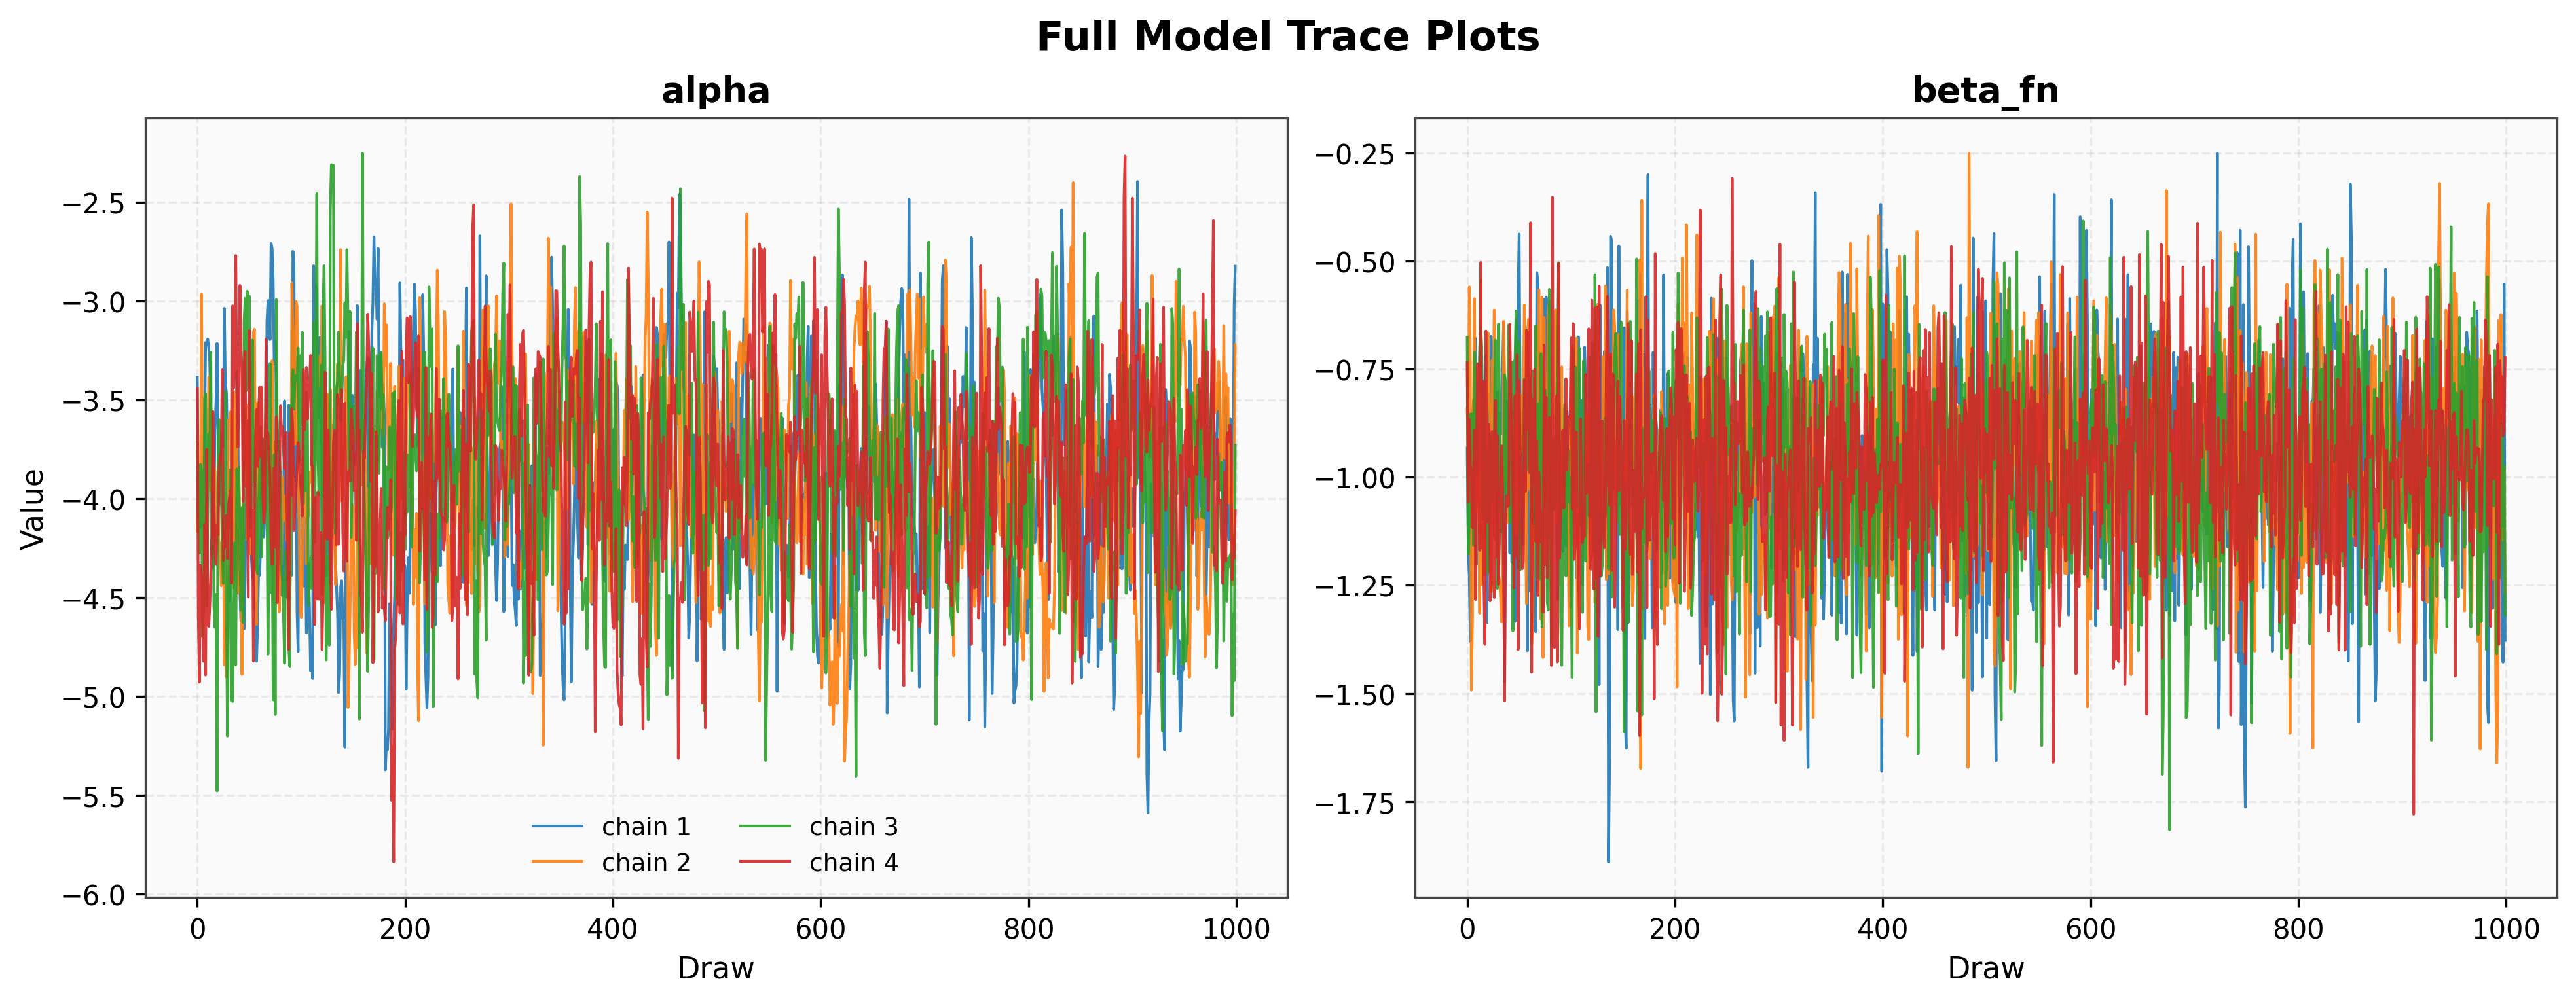
\includegraphics[width=0.92\textwidth]{figures/full_trace_alpha_beta_fn.png}\\[0.8em]
    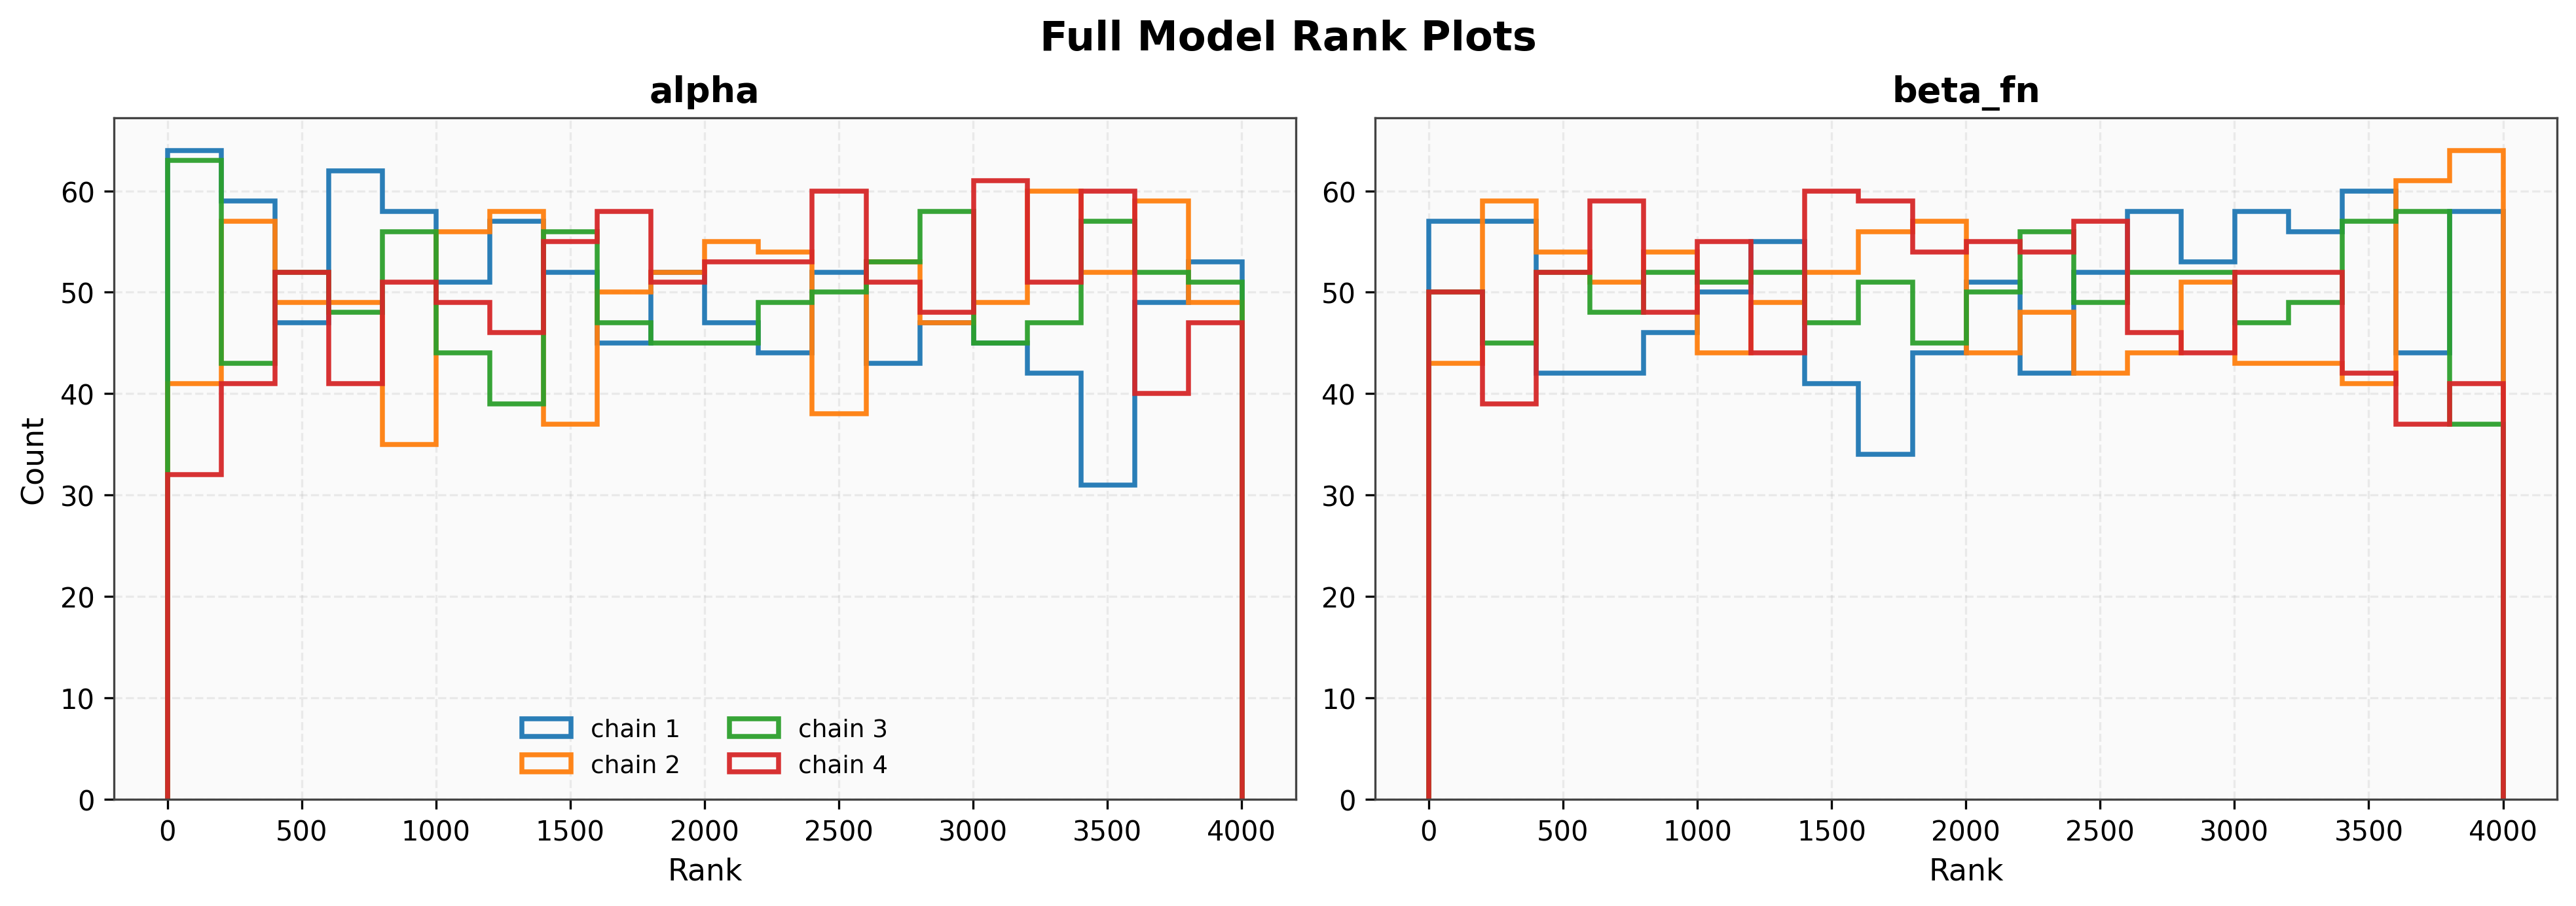
\includegraphics[width=0.92\textwidth]{figures/full_rank_alpha_beta_fn.png}
    \caption{Full-model MCMC diagnostics for parameters $\alpha$ and $\beta_{\mathrm{fn}}$: trace plots (top) and rank plots (bottom). Plots indicate fast mixing and stable estimations of parameter values.}
    \label{fig:full_trace_rank}
\end{figure}

\section{Sensitivity Analysis}\label{sec:sensitivity_analysis}

Sensitivity analysis was done only on the Province model with 3 different prior parameter settings for reasons of computational cost. The results are summarised in Table XX below.

\section{Example Stan Code}\label{sec:stan_code}

Below is the Stan code used for the Minimal model. Note that full code for all models, compilation and analysis can be found on Github\footnote{https://github.com/PierreRL/Wildfire\_Evacuations}.
\begin{verbatim}
data {
  int<lower=1> N;
  array[N] int<lower=0, upper=1> y;
  vector[N] log_fire_size;
  array[N] int<lower=0, upper=1> fn_indicator;
}

parameters {
  real alpha;
  real beta_log_fire_size;
  real beta_fn;
}

model {
  vector[N] theta;

  // Priors
  alpha ~ normal(0, 2);
  beta_log_fire_size ~ normal(0, 1);
  beta_fn ~ normal(0, 1);

  for (n in 1:N) {
    theta[n] = alpha
             + beta_log_fire_size * log_fire_size[n]
             + beta_fn * fn_indicator[n];
  }

  // Likelihood
  y ~ bernoulli_logit(theta);
}

generated quantities {
  vector[N] log_lik;
  array[N] int y_rep;

  for (n in 1:N) {
    real theta_n = alpha
                   + beta_log_fire_size * log_fire_size[n]
                   + beta_fn * fn_indicator[n];
    log_lik[n] = bernoulli_logit_lpmf(y[n] | theta_n);
    y_rep[n] = bernoulli_logit_rng(theta_n);
  }
}
\end{verbatim}

